\documentclass[10pt,conference,compsoc]{IEEEtran}

\usepackage{amsmath}
\usepackage{bm}
\usepackage{float}
\usepackage{graphicx}
\PassOptionsToPackage{hyphens}{url}\usepackage[colorlinks=true,linkcolor=blue]{hyperref}
\usepackage{tabulary}
\usepackage{tocbibind}

% Load after hyperref
\usepackage[style=super,nonumberlist,toc]{glossaries}

\makeglossaries

\newcommand{\mtx}[1] {\bm #1}

% Paper header
\usepackage{fancyhdr}
\pagestyle{fancy}
\lhead{Practical Guide to State-space Control}
\rhead{\thepage}
\lfoot{}
\rfoot{}
\fancyfoot[C]{} % remove normal page numbers

\allowdisplaybreaks

\begin{document}
\input{INP-00-glossary}

\begin{titlepage}
  \begin{center}
    \vspace*{1cm}

    \Huge
    \textbf{Practical Guide to State-space Control}

    \vspace{0.5cm}
    \LARGE
    Graduate-level control theory for high schoolers

    \vspace{1.5cm}

    \textbf{Tyler Veness}

    \vfill

    \vspace{0.8cm}

    %\begin{figure}[H]
    %  \centering
    %  \def\svgwidth{0.25\columnwidth}
    %  \input{wpilib.pdf_tex}
    %\end{figure}
  \end{center}

  \vfill

  \section{Abstract}

  \noindent Control theory is a discipline that deals with the behavior of
  dynamical \glspl{system} with inputs, and how their behavior is modified by
  feedback. Concepts from classical and modern control are introduced, and
  advice is given on when and now to use these tools.

  \section{Intended Audience}

  \noindent This guide is intended to make an advanced engineering topic
  approachable so it can be applied by those who aren't experts in control
  theory. My intended audience is high school students who are returning veteran
  members of a FIRST Robotics Competition team. As such, they will already be
  familiar with feedback control applications like PID and have basic
  proficiency in programming. This guide will build on their current knowledge
  of control theory and teach them enough about state-space control to be able
  to implement it in the programming language of their choice.

  \section{Style guide}

  \noindent This document follows the IEEE conference paper format.

  \vspace{0.8cm}
\end{titlepage}
\thispagestyle{empty}  % no page number on title sheet

\pagenumbering{roman}
\tableofcontents
\listoffigures
\listoftables
\clearpage

\pagenumbering{arabic}

\section{Preface}

\noindent I am the software mentor for a FIRST Robotics Competition team. My
responsibilities for that include teaching programming, software engineering
practices, and applications of control theory. The curriculum I developed so far
(located at \url{https://csweb.frc3512.com/ci/}) teaches rookies enough to be
minimally competitive, but many of the more advanced sections are incomplete. It
provides no formal avenues of growth for veteran students. \\

\noindent This project expands my curriculum to cover control theory topics I
have learned in my graduate-level engineering classes at University of
California, Santa Cruz. It introduces state-space controllers and serve as a
practical guide for formulating and implementing them. State-space control is a
way of formulating control problems using linear algebra that has several
advantages over simpler, typically heuristic approaches like
Proportional-Integral-Derivative (PID). \\

\noindent The sections on classical control theory are intended to provide a
geometric intuition into the mathematical machinery. Some topics have been
oversimplified to make them easier to grasp. For more detail, please see the
Wikibook on control systems at \url{https://en.wikibooks.org/wiki/Control_Systems}.

\section{What is control theory?}

\noindent How can we prove an autonomous car will behave safely? Control theory
is used to analyze and predict \gls{system} behavior. It's a pragmatic
application of algebra, geometry, and jargon with the goal of producing a
desired \gls{system} response. Feedback control facilitates producing a desired
\gls{system} response. Control theory involves judiciously expending engineering
effort to meet performance specifications.

\section{Nomenclature}

\noindent Most resources for advanced engineering topics assume a level of
knowledge well above that which is necessary. See the glossary for a list of
words and phrases commonly used in control theory, their origins, and their
meaning. \\

\noindent For example, the \gls{state} for a DC brushed motor would include the
angular velocity $\dot{\theta}$ and current $i$. Voltage $V$ is an input. With
perfect knowledge of the angular velocity and current, all future \glspl{state}
of the \gls{system} can be predicted given an input voltage signal. \\

\section{Control system diagrams}

\subsection{What is gain?}

\noindent Gain is a proportional value that shows the relationship between the
magnitude of the input to the magnitude of the output signal at steady state.
Many \glspl{system} contain a method by which the gain can be altered, providing
more or less "power" to the \gls{system}. However, increasing gain or decreasing
gain beyond a particular safety zone can cause the \gls{system} to become
unstable.

\subsection{Block diagrams}

\noindent When designing or analyzing a control system, it is useful to model it
graphically. Block diagrams are used for this purpose. They can be manipulated
and simplified systematically \cite{bib:block_diagrams}. Figure
\ref{fig:feedback_loop} is an example of one with a feedback configuration.

\begin{figure}[H]
  \centering
  \def\svgwidth{0.5\columnwidth}
  \input{Feedback_Loop.pdf_tex}
  \caption{Feedback block diagram}
  \label{fig:feedback_loop}
\end{figure}

\section{Review of PID controller mathematics}

\subsection{PID basics and theory}

\noindent Negative feedback loops drive the difference between \gls{reference}
and \gls{output} to zero. \\

\noindent \textbf{Proportional} gain compensates for current \gls{error}. \\
\textbf{Integral} gain compensates for past error (i.e.,
\gls{steady-state error}). \\
\textbf{Derivative} gain compensates for future error by slowing controller down
  if error decreases over time.

\begin{figure}[H]
  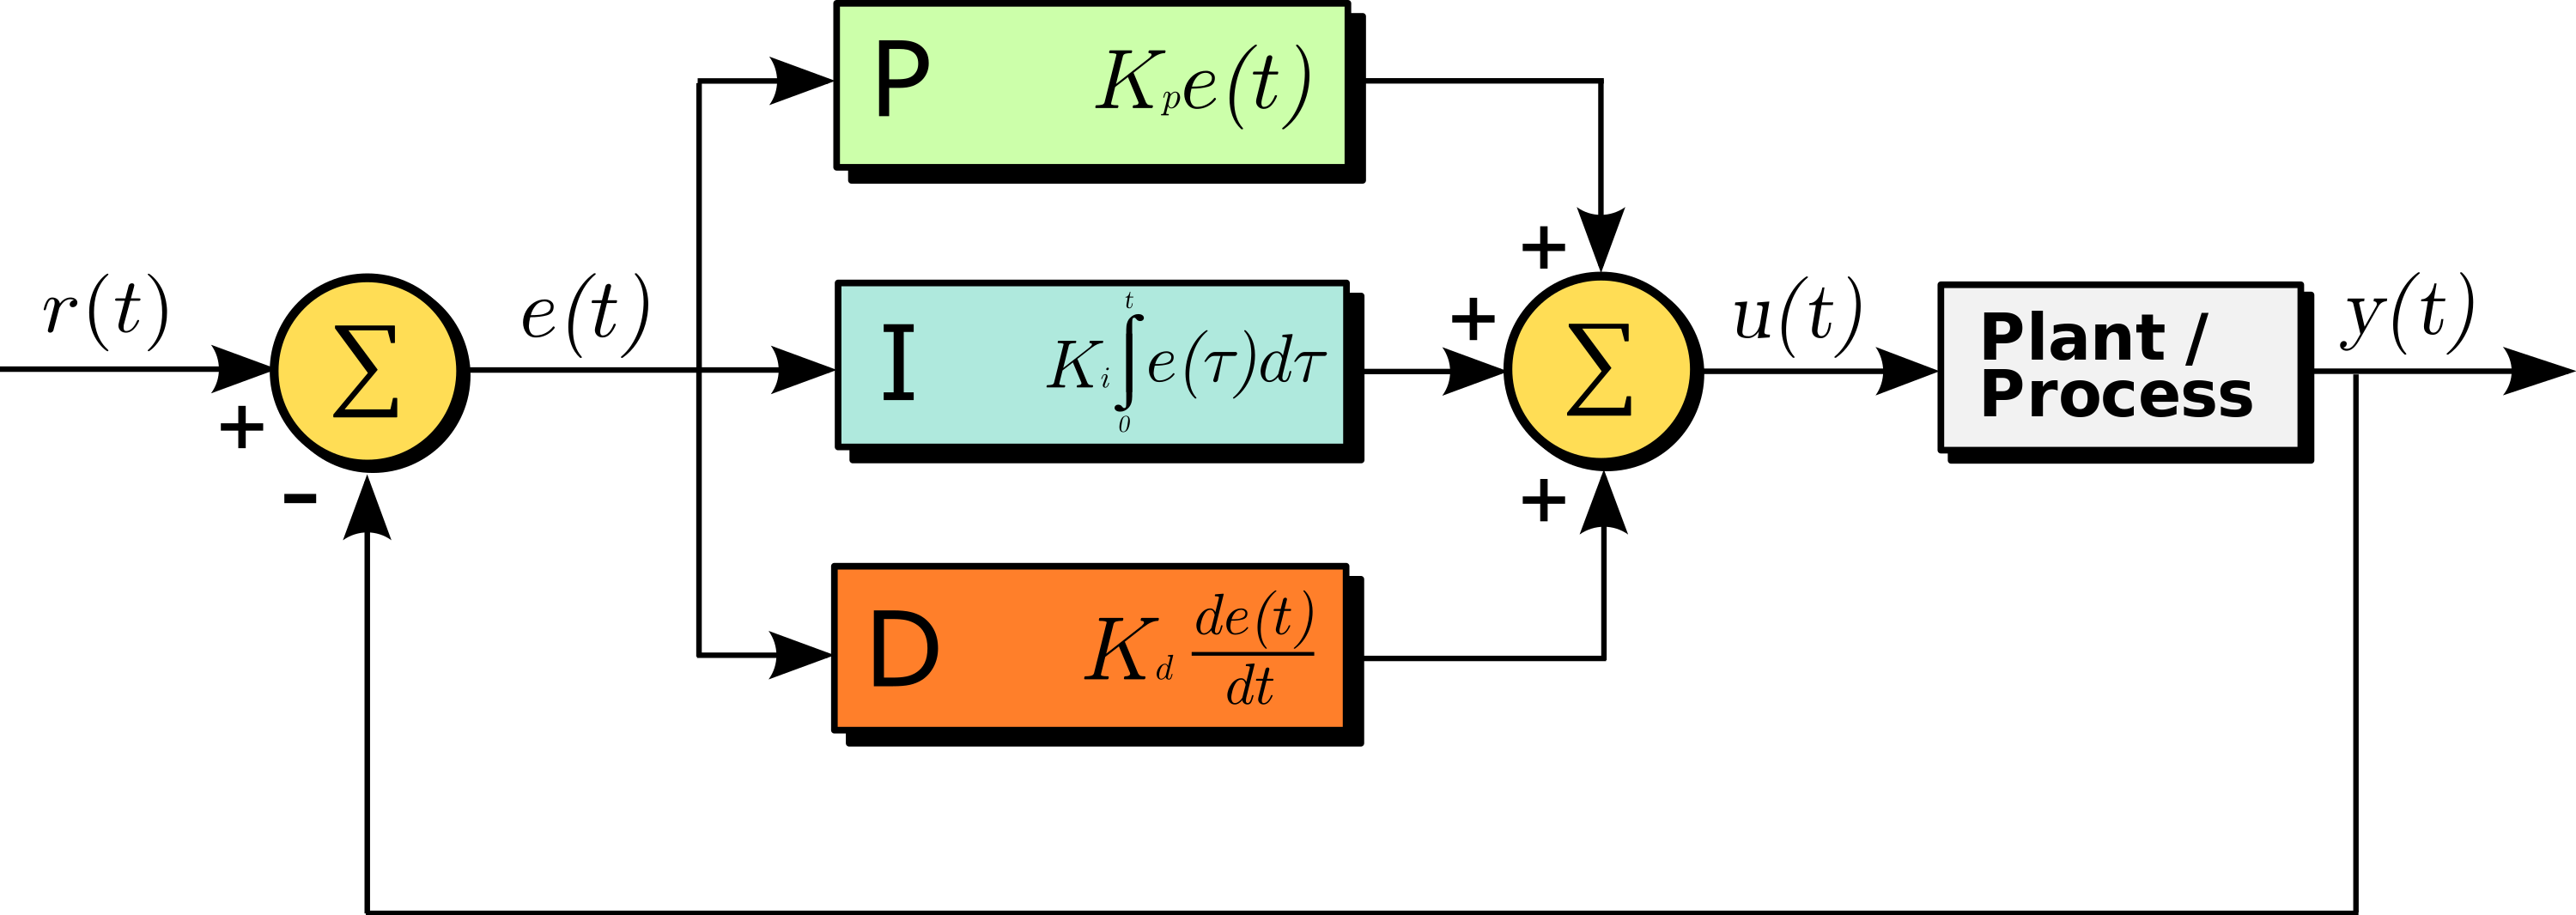
\includegraphics[width=\linewidth]{figs/PID_diagram.png}
  \caption{PID controller diagram \cite{bib:PID_diagram}}
  \label{fig:pid_ctrl_diag}
\end{figure}

\begin{table}[ht]
  \renewcommand{\arraystretch}{1.3}
  \centering
  \begin{tabulary}{\linewidth}{LLLL}
    $r(t)$ & \gls{reference} input & $u(t)$ & control input \\
    $e(t)$ & error & $y(t)$ & \gls{output} \\
  \end{tabulary}
  \label{tab:pid_def}
\end{table}

\begin{table}[ht]
  \caption{Plant versus controller}
  \renewcommand{\arraystretch}{1.3}
  \centering
  \begin{tabular}{|l|ll|}
    \hline
    & \textbf{Plant} & \textbf{Controller} \\
    \hline
    Input & $u(t)$ & $r(t)$, $y(t)$ \\
    Output & $y(t)$ & $u(t)$ \\
    \hline
  \end{tabular}
  \label{tab:plant_v_controller}
\end{table}

\subsection{Types of PID controllers}

\noindent PID controller inputs of different orders of derivatives, such as
position and velocity, affect the \gls{system} response differently. The
position PID controller is defined as

\begin{equation}
  u(t) = K_p e(t) + K_i \int_0^t e(\tau) d\tau + K_d \frac{de}{dt} \\
\end{equation}
\\
\noindent If a velocity is passed instead, which is a change in position, the
equation becomes

\begin{align}
  \frac{du}{dt} &= K_p \frac{de}{dt} + K_i \int_0^t \frac{de}{d\tau} d\tau +
    K_d \frac{d^2e}{dt^2} \nonumber \\
  \frac{du}{dt} &= K_p \frac{de}{dt} + K_i e(t) + K_d \frac{d^2e}{dt^2}
    \label{eq:pid_vel}
\end{align}
\\
\noindent This shows that $K_i$ and $K_p$ from the position controller act as
proportional and derivative terms respectively in the velocity controller. $K_i$
from the position controller has no equivalent in the velocity controller. If we
were to implement one, it would use a double integral. However, it would be of
limited use since the $K_i$ term in equation (\ref{eq:pid_vel}) also eliminates
steady-state error for step changes in \gls{reference}. Relabelling the
coefficients to match the position PID controller gives

\begin{equation}
  \frac{du}{dt} = K_p \int_0^t e(\tau) d\tau + K_d e(t) \\
\end{equation}
\\
\noindent Read \url{https://en.wikipedia.org/wiki/PID_controller} for more
information.

\subsection{Limitations of PID control}

\noindent PID's hueristic method of tuning is fine when there is no knowledge of
the \gls{system}. However, controllers with much better response can be
developed if a dynamical model of the \gls{system} is known.

\section{What is a transfer function?}

\noindent A transfer function maps an input to an output in the Laplace domain.
This is essentially a two-dimensional frequency domain on the complex plane
(real numbers on the x-axis and imaginary numbers on the y-axis). These can be
obtained by applying the Laplace transform to a differential equation and
rearranging the terms to obtain a ratio of the output variable to the input
variable. Equation \ref{eq:transfer_func} is an example of a transfer function.

\begin{equation} \label{eq:transfer_func}
  H(s) = \frac{(s-9+9i)(s-9+9i)}{s(s+10)} \\
\end{equation}

\noindent Roots of the numerator and denominator are called residues. Residues
on the top are called zeroes while residues on the bottom are called poles. This
is due to poles making the expression approach infinity for values of $s$ that
make the residue zero (they look like poles of a circus tent on a 3D graph).
Similar logic applies to zeroes. Imaginary roots always come in complex
conjugate pairs (e.g., $-2 + 3i$, $-2 - 3i$).

\subsection{Transfer functions in feedback}

\noindent For \glspl{controller} to perform their job, they must be placed in
feedback. attempt to bring about a desired \gls{system} state by
driving the difference between a \gls{reference} signal and the \gls{output} to
zero. This is done by placing the controller and \gls{plant} in feedback. For
example, the transfer function of figure \ref{fig:feedback_loop} from input to
output is

\begin{equation}
  G_{cl}(s) = \frac{Y(s)}{X(s)} = \frac{P_1}{1 + P_1 P_2}
\end{equation}

\noindent The numerator is the \gls{open-loop gain} and the denominator is the
gain around the feedback loop, which may include parts of the
\gls{open-loop gain}. Plants are generally written with the letter $G$. As
another example, the transfer function from the input to the error is

\begin{equation}
  G_{cl}(s) = \frac{E(s)}{X(s)} = \frac{1}{1 + P_1 P_2}
\end{equation}

\noindent The roots of the denominator of $G_cl(s)$ are different from those of
the open-loop transfer function $P_1(s)$. These are called the closed-loop
poles.

\section{Location of Poles and Zeroes}

\noindent The location of the poles on the complex plane determine the stability
of the \gls{system}. Each pole represents a frequency mode of the \gls{system},
and their location determines how much of each response is induced for a given
input frequency.

\begin{figure}[H]
  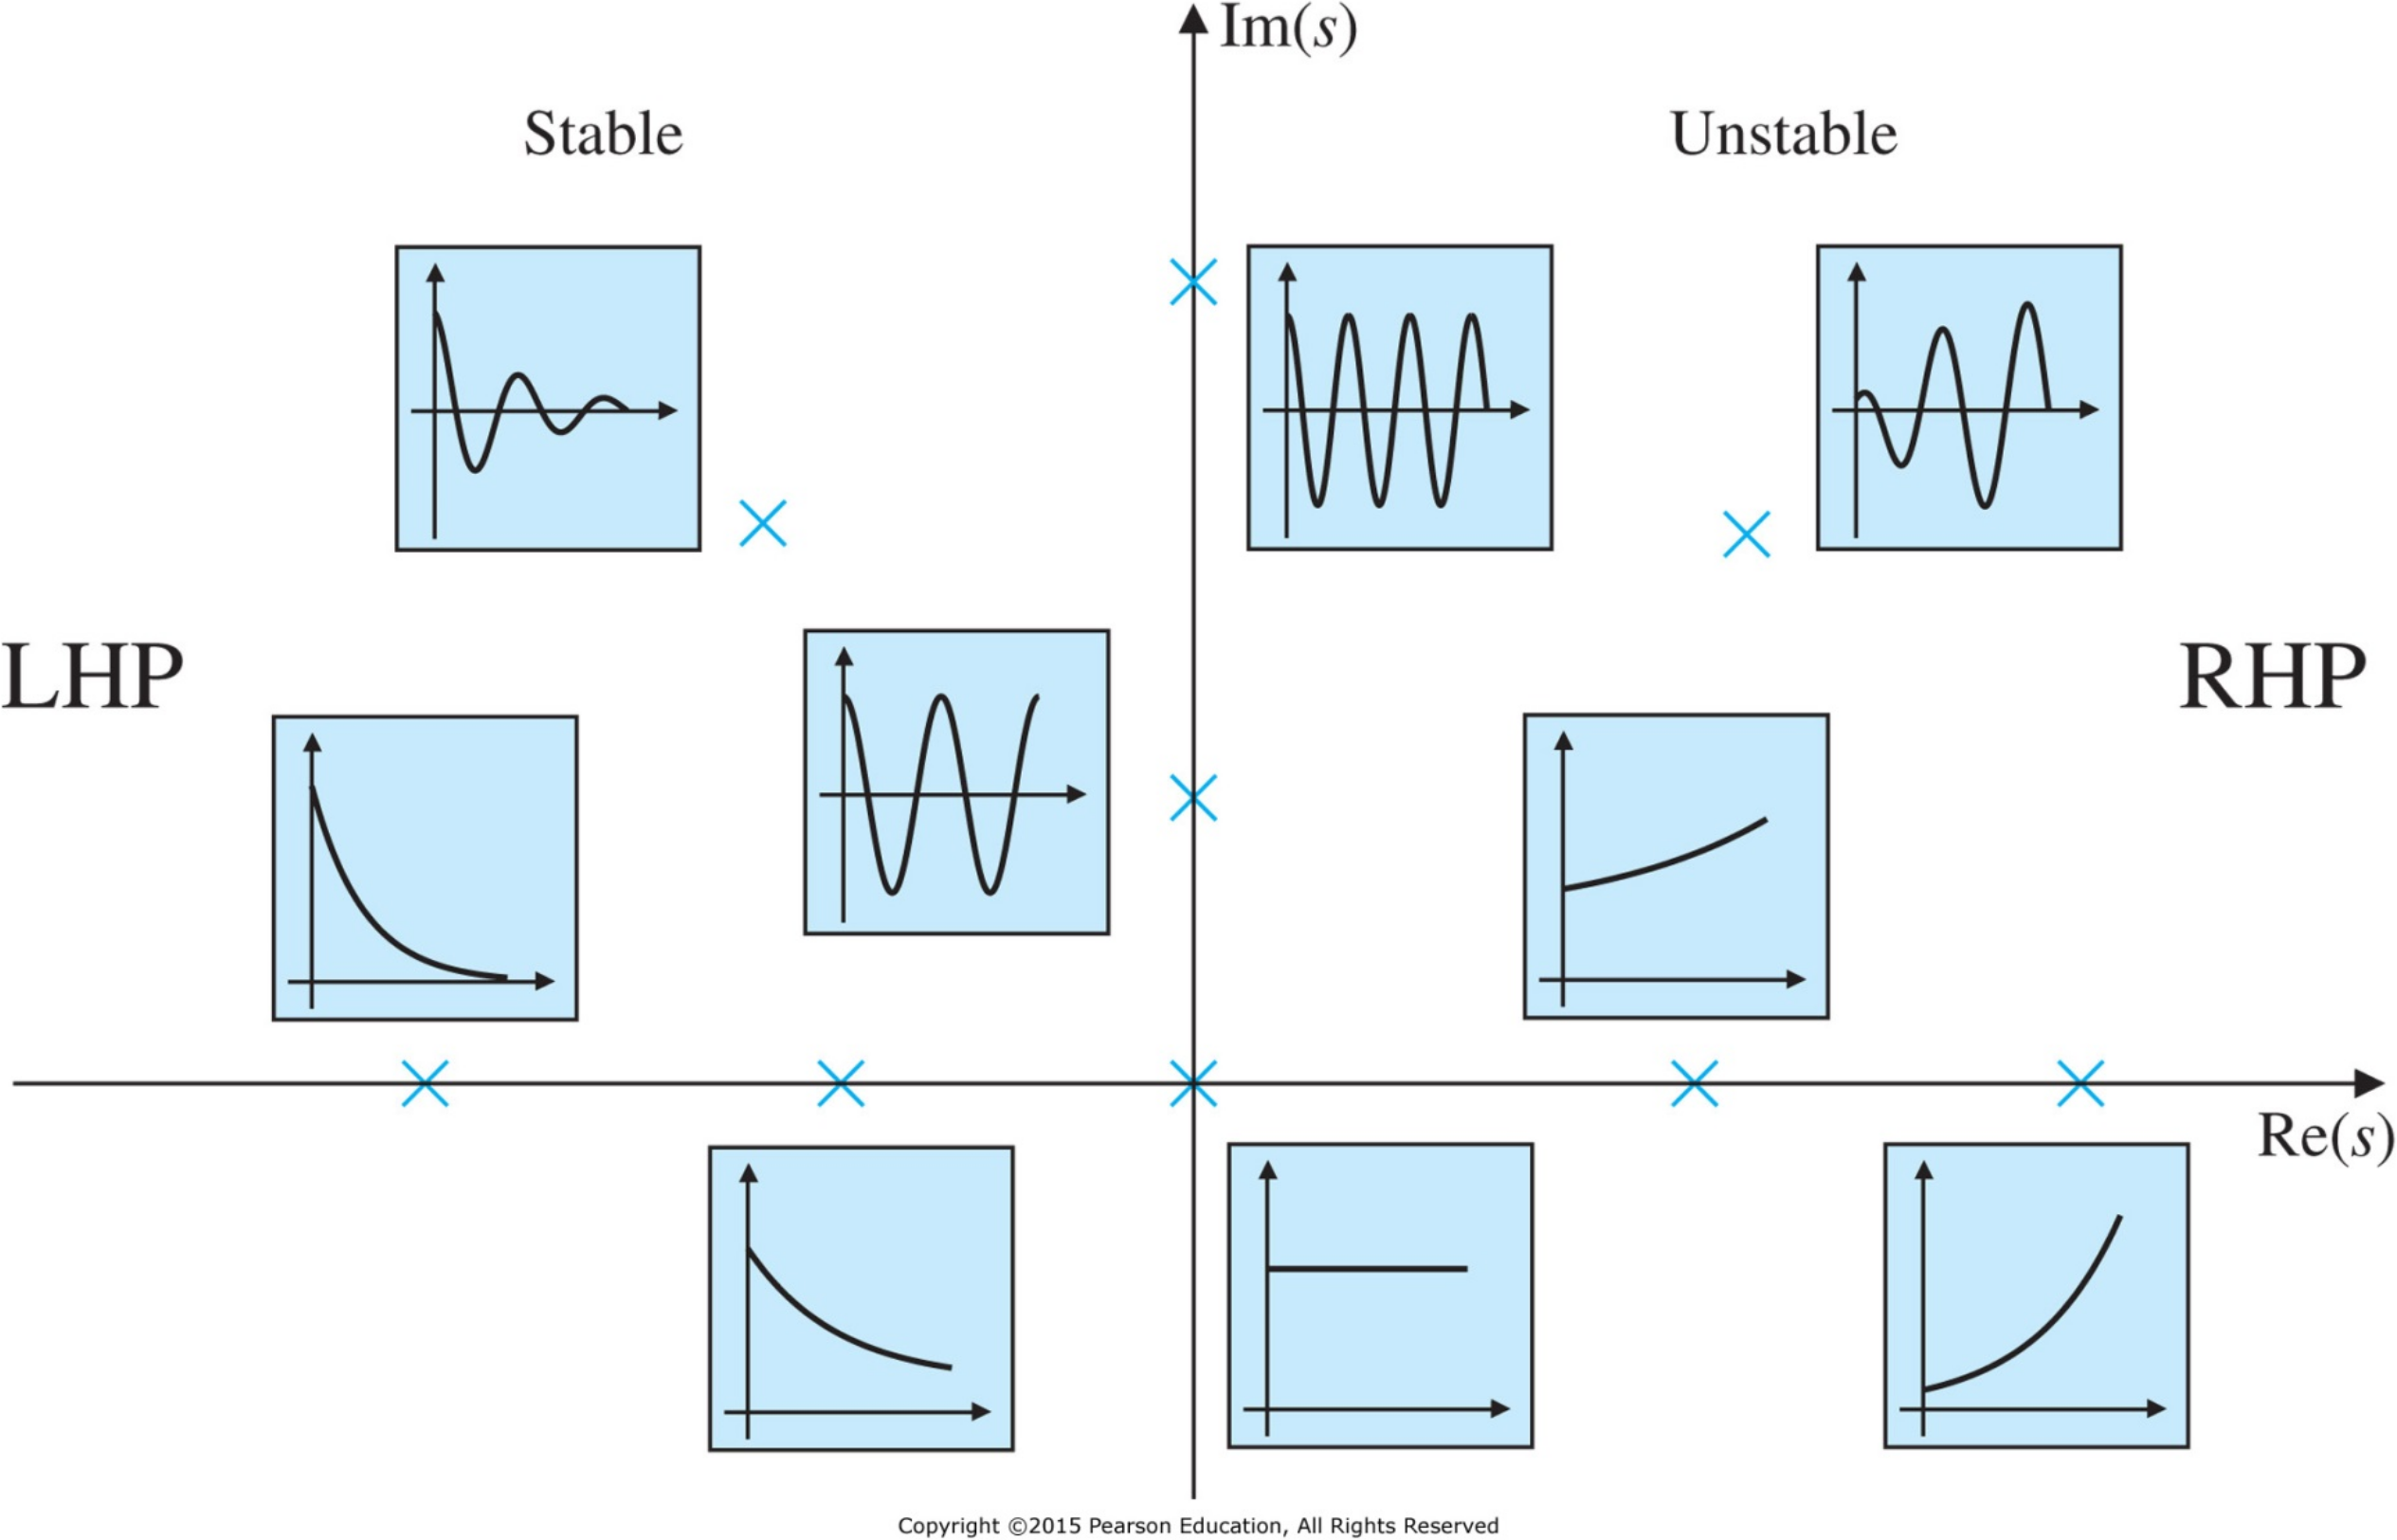
\includegraphics[width=\linewidth]{figs/ResponseVsPoleLocations.png}
  \caption{System responses vs pole locations \cite{bib:pole_locations}}
\end{figure}

\begin{table}[ht]
  \caption{Pole location and stabilty}
  \renewcommand{\arraystretch}{1.5}
  \centering
  \begin{tabular}{|ll|}
    \hline
    \textbf{Location} & \textbf{Stability} \\
    \hline
    Left-Hand Plane (LHP) & stable \\
    Imaginary Axis & marginally stable \\
    Right-Hand Plane (RHP) & unstable \\
    \hline
  \end{tabular}
  \label{tab:pole_locations}
\end{table}

\subsection{Root locus}

\noindent In closed-loop, the poles and zeroes can be moved around by the chosen
controller. The root locus shows where they will go as the controller gain is
increased. Figure \ref{fig:poster_rlocus} shows the root locus of the transfer
function from equation (\ref{eq:transfer_func}).

\begin{figure}[H]
  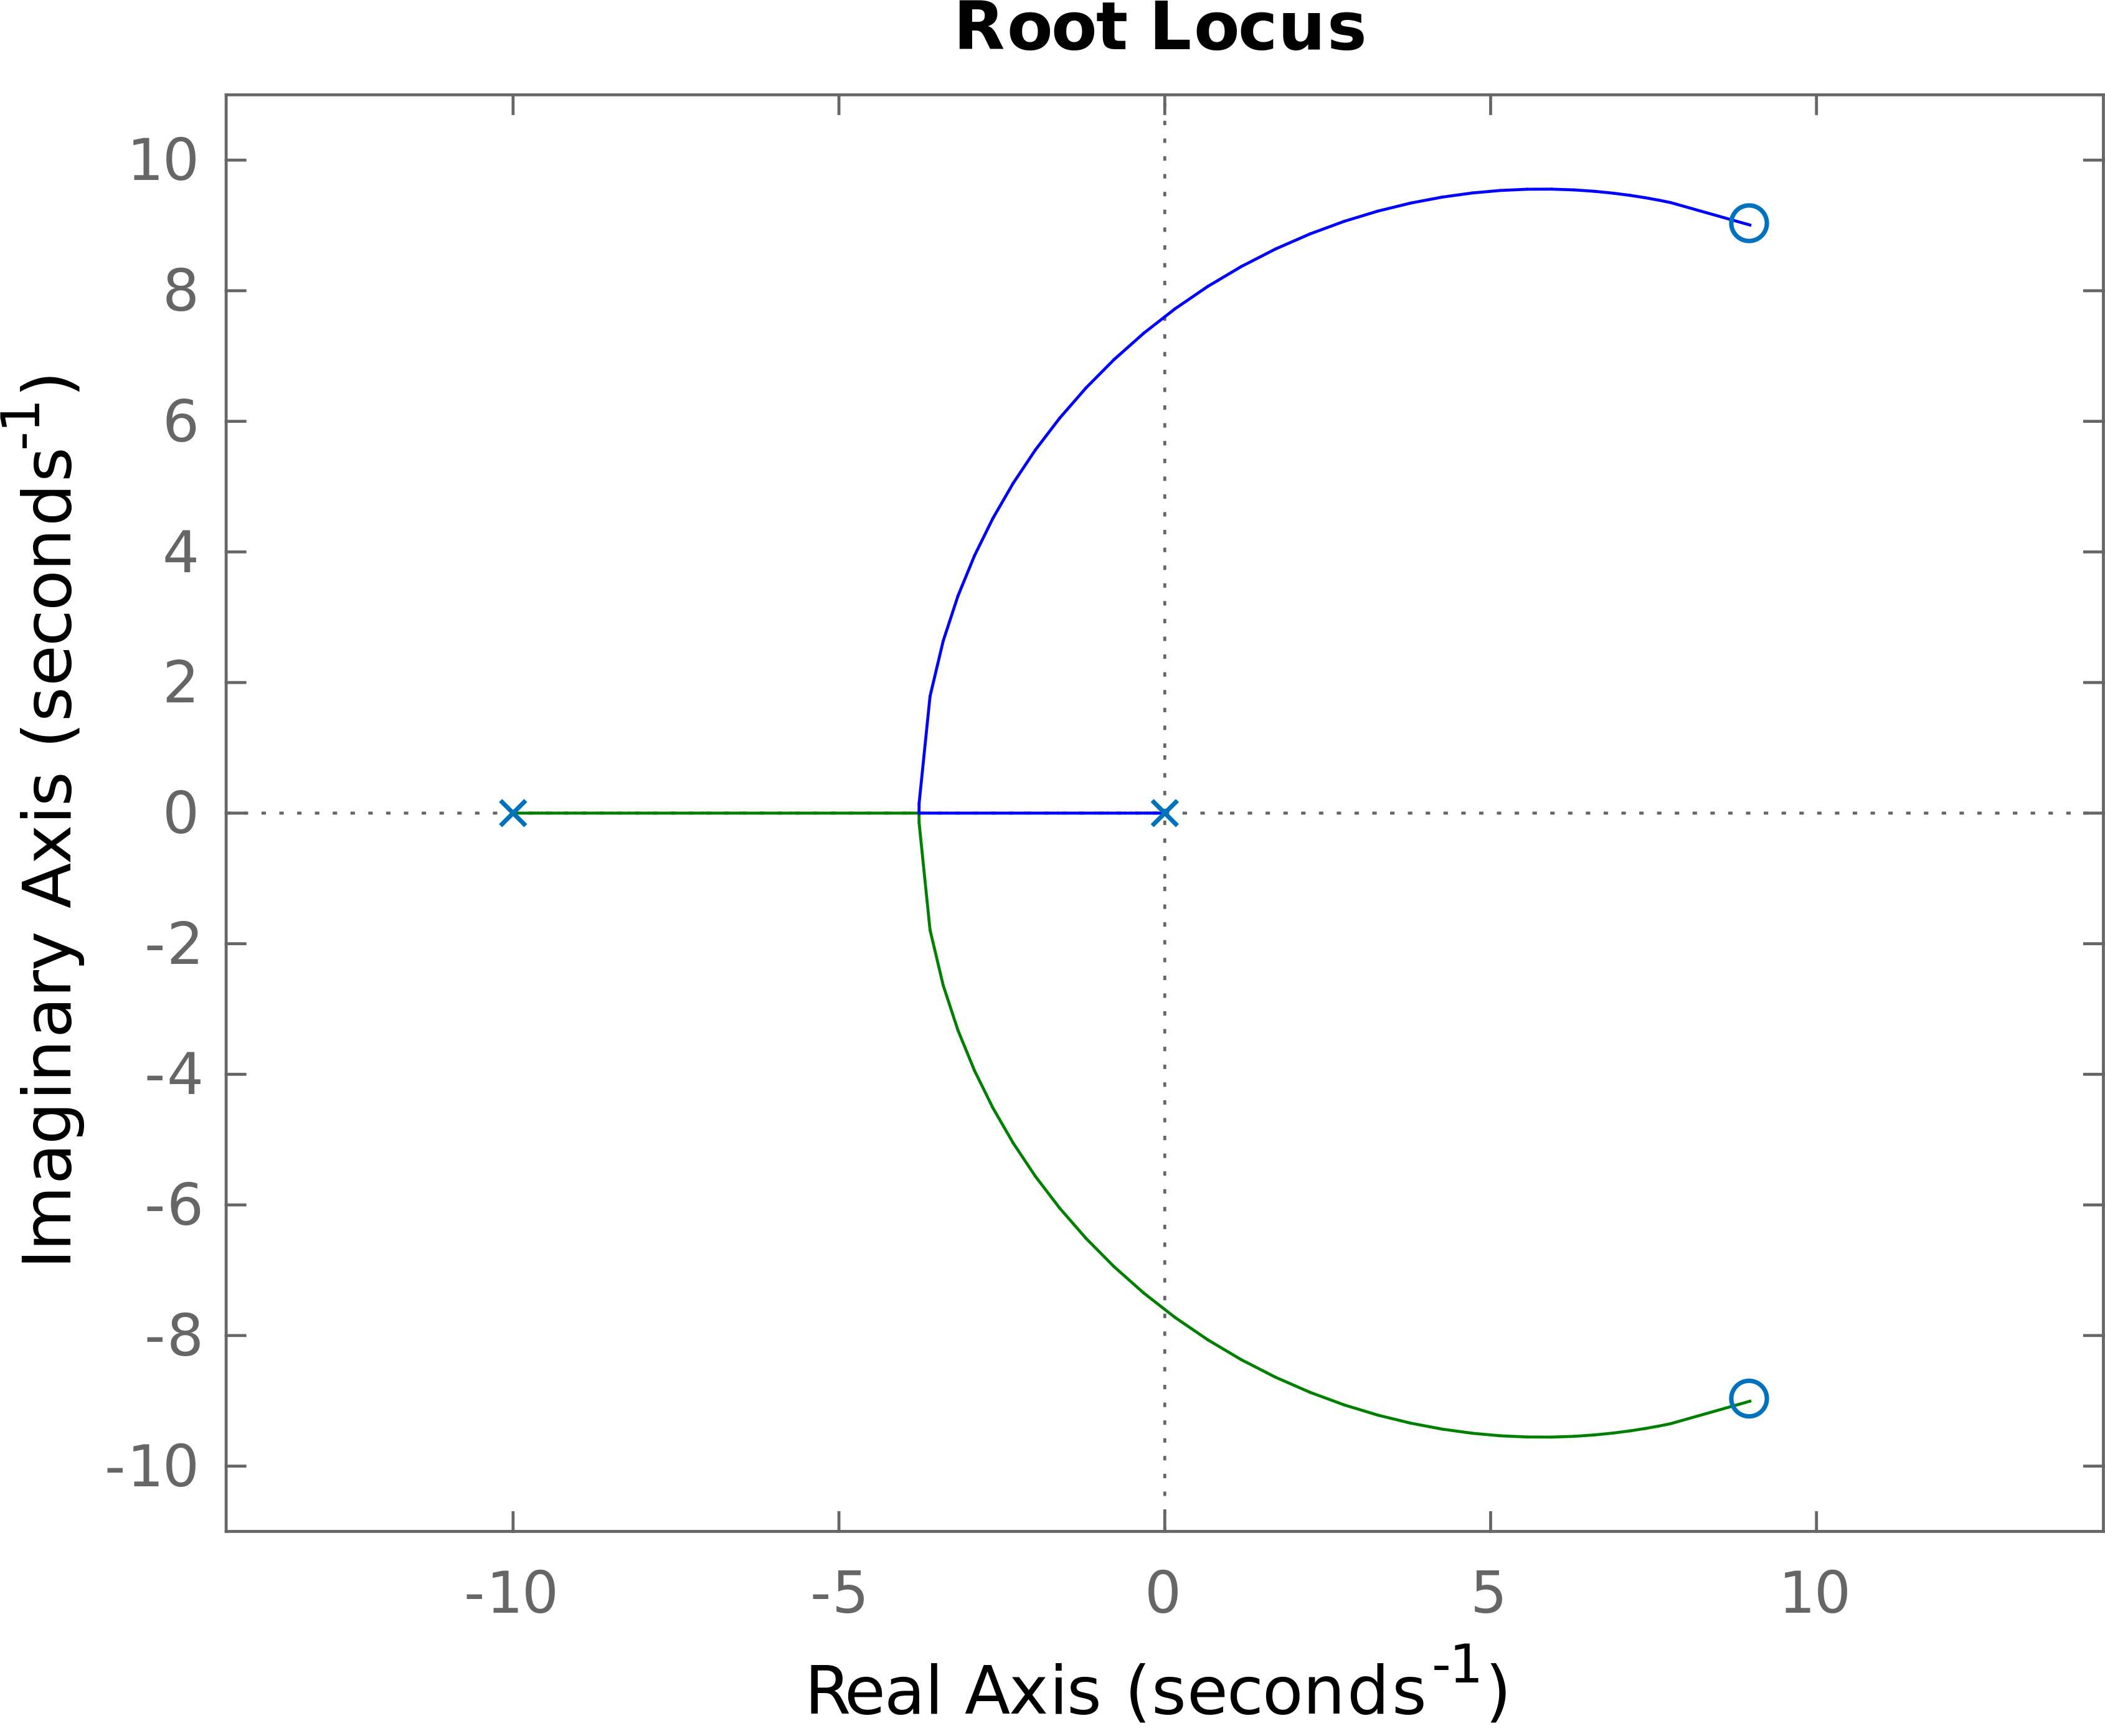
\includegraphics[width=\linewidth]{figs/poster_rlocus.png}
  \caption{Root locus of equation (\ref{eq:transfer_func})}
  \label{fig:poster_rlocus}
\end{figure}

\noindent As the controller gain increases, the poles move toward the zeroes. In
this case, the \gls{system} eventually becomes unstable. \\

\noindent \textbf{Note:} If poles are much farther left in the LHP than the
typical \gls{system} dynamics exhibit, they can be considered negligible. Every
\gls{system} has some form of unmodeled high frequency, non-linear dynamics, but
they can be safely ignored depending on the operating regime.

\subsubsection{Non-minimum phase zeroes}

While poles in the RHP are unstable, the same is not true for zeroes. They can
be characterized by the \gls{system} initially moving in the wrong direction
before heading toward the \gls{reference}. Since the poles always move toward
the zeroes, zeroes impose a "speed limit" on the \gls{system} response because
it takes a finite amount of time to move the wrong direction, then change
directions. \\

\noindent One example is bicycle steering. Try riding a bicycle without holding
the handle bars, then poke the right handle; the bicycle turns right.

\section{Steady-state error}

\noindent To demonstrate the problem of \gls{steady-state error}, we will use a
DC brushed motor controlled by a velocity PID controller. A DC brushed motor has
a transfer function from voltage ($V$) to angular velocity ($\dot{\theta}$) of

\begin{equation}
  G(s) = \frac{\dot{\Theta}(s)}{V(s)} = \frac{K}{(Js+b)(Ls+R)+K^2} \\
\end{equation}

\noindent First, we'll try controlling it with a P controller defined as

\begin{equation*}
  K(s) = K_p \\
\end{equation*}

\noindent When these are in unity feedback, the transfer function from the input
voltage to the error is

\begin{align*}
  \frac{E(s)}{V(s)} &= \frac{1}{1 + K(s)G(s)} \\
  E(s) &= \frac{1}{1 + K(s)G(s)} V(s) \\
  E(s) &= \frac{1}{1 + (K_p) \left(\frac{K}{(Js+b)(Ls+R)+K^2}\right)} V(s) \\
  E(s) &= \frac{1}{1 + \frac{K_p K}{(Js+b)(Ls+R)+K^2}} V(s)
\end{align*}

The steady-state of a transfer function can be found via

\begin{equation}
  \lim_{s\to0} sH(s)
\end{equation}

\begin{align}
  e_{ss} &= \lim_{s\to0} sE(s) \nonumber \\
  e_{ss} &= \lim_{s\to0} s \frac{1}{1 + \frac{K_p K}{(Js+b)(Ls+R)+K^2}} V(s)
    \nonumber \\
  e_{ss} &= \lim_{s\to0} s \frac{1}{1 + \frac{K_p K}{(Js+b)(Ls+R)+K^2}}
    \frac{1}{s} \nonumber \\
  e_{ss} &= \lim_{s\to0} \frac{1}{1 + \frac{K_p K}{(Js+b)(Ls+R)+K^2}}
    \nonumber \\
  e_{ss} &= \frac{1}{1 + \frac{K_p K}{(J(0)+b)(L(0)+R)+K^2}} \nonumber \\
  e_{ss} &= \frac{1}{1 + \frac{K_p K}{bR+K^2}} \label{eq:ss_nonzero}
\end{align}

\noindent Notice that the \gls{steady-state error} is non-zero. To fix this, an
integrator must be included in the controller.

\begin{equation*}
  K(s) = K_p + \frac{K_i}{s} \\
\end{equation*}

\noindent The same steady-state calculations are performed as before with the
new controller.

\begin{align*}
  \frac{E(s)}{V(s)} &= \frac{1}{1 + K(s)G(s)} \\
  E(s) &= \frac{1}{1 + K(s)G(s)} V(s) \\
  E(s) &= \frac{1}{1 + \left(K_p + \frac{K_i}{s}\right)
    \left(\frac{K}{(Js+b)(Ls+R)+K^2}\right)} \left(\frac{1}{s}\right) \\
  e_{ss} &= \lim_{s\to0} s \frac{1}{1 + \left(K_p + \frac{K_i}{s}\right)
    \left(\frac{K}{(Js+b)(Ls+R)+K^2}\right)} \left(\frac{1}{s}\right) \\
  e_{ss} &= \lim_{s\to0} \frac{1}{1 + \left(K_p + \frac{K_i}{s}\right)
    \left(\frac{K}{(Js+b)(Ls+R)+K^2}\right)} \\
  e_{ss} &= \lim_{s\to0} \frac{1}{1 + \left(K_p + \frac{K_i}{s}\right)
    \left(\frac{K}{(Js+b)(Ls+R)+K^2}\right)} \frac{s}{s} \\
  e_{ss} &= \lim_{s\to0} \frac{s}{s + \left(K_p s + K_i\right)
    \left(\frac{K}{(Js+b)(Ls+R)+K^2}\right)} \\
  e_{ss} &= \frac{0}{0 + (K_p (0) + K_i)
    \left(\frac{K}{(J(0)+b)(L(0)+R)+K^2}\right)} \\
  e_{ss} &= \frac{0}{K_i \frac{K}{bR+K^2}} \\
\end{align*}

\noindent The denominator is non-zero, so $e_{ss} = 0$. Therefore, an integrator
is required to eliminate \gls{steady-state error} in all cases for this model.
\\

\noindent It should be noted that $e_{ss}$ in equation (\ref{eq:ss_nonzero})
tends to zero for $K_p = \infty$. This is known as a bang-bang controller. In
practice, an infinite switching frequency cannot be achieved, but it may be
close enough for some performance specifications.

\section{Going Digital}

\noindent The complex plane discussed so far deals with continuous
\glspl{system}. In decades past, \glspl{plant} and controllers were implemented
using analog electronics, which are continuous in nature. Nowadays,
microprocessors can be used to achieve cheaper, less complex controller designs.
However, this comes with drawbacks. \\

\noindent Since a microcontroller performs discrete steps, there is phase loss
introduced in the controller. Large amounts of phase loss can make a stable
controller in the continuous domain go unstable in discrete. Here are a few ways
to combat this.

\begin{itemize}
  \item Run the controller with a high sample rate.
  \item Designing the controller in the analog domain with enough phase margin to compensate for any phase loss that occurs as part of discretization.
  \item Convert the \gls{plant} to the digital domain and design the controller
    completely in the digital domain.
\end{itemize}

\subsection{s-plane to z-plane}

\noindent Transfer functions are converted to impulse responses using the
Z-transform. The s-plane's LHP maps to the inside of a unit circle in the
z-plane. Here are a few common points.

\begin{table}[ht]
  \caption{Mapping from s-plane to z-plane}
  \renewcommand{\arraystretch}{1.3}
  \centering
  \begin{tabular}{|cc|}
    \hline
    \textbf{s-plane} & \textbf{z-plane} \\
    \hline
    $(0, 0)$ & $(0, 1)$ \\
    imaginary axis & edge of unit circle \\
    $(0, -\infty)$ & $(0, 0)$ \\
    \hline
  \end{tabular}
  \label{tab:s-plane2z-plane}
\end{table}

\noindent You may notice that poles can be placed at $(0, 0)$ in the z-plane.
This is known as a deadbeat controller. An $\rm N^{th}$ order deadbeat controller
decays to the \gls{reference} in N timesteps. While this sounds great, there are
other considerations like actuation effort and robustness. These will be
discussed in detail with LQR controllers.

\section{Linear algebra}

\noindent Modern control theory borrows concepts from linear algebra. We
recommend watching 3Blue1Brown's \textit{Essence of Linear Algebra} video series
\cite{bib:essence_of_linalg}. It offers an intuitive, geometric understanding of
linear algebra as a method of linear transformations.

\section{State-space}

\noindent A state-space representation models \glspl{system} as a set of
\gls{state}, input, and output variables related by first-order differential
equations. "State space" refers to the Euclidean space in which the \gls{state}
variables are on the axes. The \gls{state} of the \gls{system} can be
represented as a vector within that space. \\

\noindent To abstract from the number of \glspl{state}, inputs, and outputs,
these variables are expressed as vectors. Additionally, if the dynamical
\gls{system} is linear, time-invariant, and finite-dimensional, then the
differential and algebraic equations may be written in matrix form.

\subsection{Benefits over classical output-based control}

\noindent The state-space method is characterized by significant algebraization
of general system theory. The state-space representation uses the time domain
instead of the frequency domain, and provides a convenient and compact way to
model and analyze \glspl{system} with multiple inputs and outputs. With $p$
inputs and $q$ outputs, we would otherwise have to write down $q \times p$
Laplace transforms to encode all the information about a system. Unlike the
frequency domain approach, the use of the state-space representation is not
limited to systems with linear components and zero initial conditions.

\subsection{Optimal control techniques}

\section{State-space notation}

\begin{align}
  \dot{\mtx{x}} &= \mtx{A}\mtx{x} + \mtx{B}\mtx{u} \label{eq:s_ctrl_x} \\
  \mtx{y} &= \mtx{C}\mtx{x} + \mtx{D}\mtx{u} \label{eq:s_ctrl_y}
\end{align}

\begin{align}
  \mtx{x}_{k+1} &= \mtx{A}\mtx{x}_k + \mtx{B}\mtx{u}_k \label{eq:z_ctrl_x} \\
  \mtx{y}_{k+1} &= \mtx{C}\mtx{x}_k + \mtx{D}\mtx{u}_k \label{eq:z_ctrl_y}
\end{align}

\begin{table}[ht]
  \renewcommand{\arraystretch}{1.3}
  \centering
  \begin{tabulary}{\linewidth}{LLLL}
    $\mtx{A}$ & system matrix      & $\mtx{x}$ & state vector \\
    $\mtx{B}$ & input matrix       & $\mtx{u}$ & input vector \\
    $\mtx{C}$ & output matrix      & $\mtx{y}$ & output vector \\
    $\mtx{D}$ & feedthrough matrix & $\mtx{K}$ & controller gain matrix \\
  \end{tabulary}
  \label{tab:ctrl_def}
\end{table}

\section{Canonical forms}

\subsection{Controllable Canonical Form}

\noindent State controllability condition implies that it is possible --
by admissible inputs -- to steer the \glspl{state} from any initial value to any
final value within some finite time window. A continuous time-invariant linear
state-space model is controllable if and only if

\begin{equation}
  rank \left[
  \begin{array}{ccccc}
    B & AB & A^2B & \cdots & A^{n-1}B
  \end{array}
  \right] = n
  \label{eq:ctrl_rank}
\end{equation}

\noindent where rank is the number of linearly independent rows in a matrix and
$n$ is the number of \gls{state} variables. \\

\noindent Given a \gls{system} of the form

\begin{equation} \label{eq:ctrl_obsv_tf}
  G(s) = \frac{n_1 s^3 + n_2 s^2 + n_3 s + n_4}
    {s^4 + d_1 s^3 + d_2 s^2 + d_3 s + d_4} \\
\end{equation}
\\
\noindent The canonical realization of it that satisfies equation
(\ref{eq:ctrl_rank}) is

\begin{align}
  \dot{\mtx{x}}(t) &= \left[
  \begin{array}{cccc}
    0 & 1 & 0 & 0 \\
    0 & 0 & 1 & 0 \\
    0 & 0 & 0 & 1 \\
    -d_4 & -d_3 & -d_2 & -d_1
  \end{array}
  \right] \mtx{x}(t) + \left[
  \begin{array}{c}
    0 \\
    0 \\
    0 \\
    1
  \end{array}
  \right] \mtx{u}(t) \\
  \mtx{y}(t) &= \left[
  \begin{array}{cccc}
    n_4 & n_3 & n_2 & n_1
  \end{array}
  \right] \mtx{x}(t)
\end{align}

\subsection{Observable Canonical Form}

\noindent Observability is a measure for how well internal \glspl{state} of a
\gls{system} can be inferred by knowledge of its external outputs. The
observability and controllability of a \gls{system} are mathematical duals
(i.e., as controllability provides that an input is available that brings any
initial \gls{state} to any desired final \gls{state}, observability provides
that knowing an output trajectory provides enough information to predict the
initial \gls{state} of the \gls{system}).

\noindent A continuous time-invariant linear state-space model is observable if
and only if

\begin{equation} \label{eq:obsv_rank}
  rank \left[
  \begin{array}{c}
    C \\
    CA \\
    \vdots \\
    CA^{n-1}
  \end{array}
  \right] = n \\
\end{equation}

\noindent The canonical realization of the \gls{system} in equation
(\ref{eq:ctrl_obsv_tf}) that satisfies equation (\ref{eq:obsv_rank}) is

\begin{align}
  \dot{\mtx{x}}(t) &= \left[
  \begin{array}{cccc}
    0 & 0 & 0 & -d_4 \\
    1 & 0 & 0 & -d_3 \\
    0 & 1 & 0 & -d_2 \\
    0 & 0 & 1 & -d_1
  \end{array}
  \right] \mtx{x}(t) + \left[
  \begin{array}{c}
    n_4 \\
    n_3 \\
    n_2 \\
    n_1
  \end{array}
  \right] \mtx{u}(t) \\
  \mtx{y}(t) &= \left[
  \begin{array}{cccc}
    0 & 0 & 0 & 1
  \end{array}
  \right] \mtx{x}(t)
\end{align}

\section{Examples}

\subsection{Spring-mass system}

\subsection{Pendulum}

\subsection{DC brushed motor}

\section{Eigenvalues in state-space}

\noindent Eigenvalues can be used to determine the stability of a \gls{system}.
\\

\noindent We'd like to know whether the \gls{system} defined by equation
(\ref{eq:z_ctrl_x}) operating with the input
$\mtx{u}_k = \mtx{K}(\mtx{R}_k - \mtx{x}_k)$ converges to the \gls{reference}
$\mtx{R}_k$.

\begin{align}
  \mtx{x}_{k+1} &= \mtx{A}\mtx{x}_k + \mtx{B}\mtx{u}_k \nonumber \\
  \mtx{x}_{k+1} &= \mtx{A}\mtx{x}_k + \mtx{B}(\mtx{K}(\mtx{R}_k - \mtx{x}_k))
    \nonumber \\
  \mtx{x}_{k+1} &= \mtx{A}\mtx{x}_k + \mtx{B}\mtx{K}\mtx{R}_k -
    \mtx{B}\mtx{K}\mtx{x}_k \nonumber \\
  \mtx{x}_{k+1} &= \mtx{A}\mtx{x}_k - \mtx{B}\mtx{K}\mtx{x}_k +
    \mtx{B}\mtx{K}\mtx{R}_k \nonumber \\
  \mtx{x}_{k+1} &= (\mtx{A} - \mtx{B}\mtx{K})\mtx{x}_k +
    \mtx{B}\mtx{K}\mtx{R}_k \label{eq:ctrl_eig_calc}
\end{align}
\\
\noindent For equation (\ref{eq:ctrl_eig_calc}) to have a bounded output, the
eigenvalues of $\mtx{A} - \mtx{B}\mtx{K}$ must be within the unit circle. \\

\noindent This derivation can be performed for a \gls{state} estimator as well
to determine whether the \gls{state} estimate converges to the real \gls{state}.
Plugging equation (\ref{eq:z_obsv_y}) into equation (\ref{eq:z_obsv_x}) gives

\begin{align*}
  \hat{\mtx{x}}_{k+1} &= \mtx{A}\hat{\mtx{x}}_k + \mtx{B}\mtx{u}_k +
    \mtx{L} (\mtx{y}_k - \hat{\mtx{y}}_{k+1}) \\
  \hat{\mtx{x}}_{k+1} &= \mtx{A}\hat{\mtx{x}}_k + \mtx{B}\mtx{u}_k +
    \mtx{L} (\mtx{y}_k - (\mtx{C}\hat{\mtx{x}}_k + \mtx{D}\mtx{u}_k)) \\
  \hat{\mtx{x}}_{k+1} &= \mtx{A}\hat{\mtx{x}}_k + \mtx{B}\mtx{u}_k +
    \mtx{L} (\mtx{y}_k - \mtx{C}\hat{\mtx{x}}_k - \mtx{D}\mtx{u}_k) \\
\end{align*}

\noindent Plugging in equation (\ref{eq:z_ctrl_y}) gives

\begin{align*}
  \hat{\mtx{x}}_{k+1} &= \mtx{A}\hat{\mtx{x}}_k + \mtx{B}\mtx{u}_k +
    \mtx{L}((\mtx{C}\mtx{x}_k + \mtx{D}\mtx{u}_k) - \mtx{C}\hat{\mtx{x}}_k -
    \mtx{D}\mtx{u}_k) \\
  \hat{\mtx{x}}_{k+1} &= \mtx{A}\hat{\mtx{x}}_k + \mtx{B}\mtx{u}_k +
    \mtx{L}(\mtx{C}\mtx{x}_k + \mtx{D}\mtx{u}_k - \mtx{C}\hat{\mtx{x}}_k -
    \mtx{D}\mtx{u}_k) \\
  \hat{\mtx{x}}_{k+1} &= \mtx{A}\hat{\mtx{x}}_k + \mtx{B}\mtx{u}_k +
    \mtx{L}(\mtx{C}\mtx{x}_k - \mtx{C}\hat{\mtx{x}}_k) \\
  \hat{\mtx{x}}_{k+1} &= \mtx{A}\hat{\mtx{x}}_k + \mtx{B}\mtx{u}_k +
    \mtx{L}\mtx{C}(\mtx{x}_k - \hat{\mtx{x}}_k) \\
\end{align*}

\noindent Let $E_k = \mtx{x}_k - \hat{\mtx{x}}_k$ be the error in the estimate
$\hat{\mtx{x}}_k$.

\begin{equation*}
  \hat{\mtx{x}}_{k+1} = \mtx{A}\hat{\mtx{x}}_k + \mtx{B}\mtx{u}_k +
    \mtx{L}\mtx{C}\mtx{E}_k \\
\end{equation*}
\\
\noindent Subtracting this from equation (\ref{eq:z_ctrl_x}) gives

\begin{align}
  \mtx{x}_{k+1} - \hat{\mtx{x}}_{k+1} &= \mtx{A}\mtx{x}_k + \mtx{B}\mtx{u}_k -
    (\mtx{A}\hat{\mtx{x}}_k + \mtx{B}\mtx{u}_k +
     \mtx{L}\mtx{C}\mtx{E}_k) \nonumber \\
  \mtx{E}_{k+1} &= \mtx{A}\mtx{x}_k + \mtx{B}\mtx{u}_k -
    (\mtx{A}\hat{\mtx{x}}_k + \mtx{B}\mtx{u}_k + \mtx{L}\mtx{C}\mtx{E}_k)
    \nonumber \\
  \mtx{E}_{k+1} &= \mtx{A}\mtx{x}_k + \mtx{B}\mtx{u}_k -
    \mtx{A}\hat{\mtx{x}}_k - \mtx{B}\mtx{u}_k - \mtx{L}\mtx{C}\mtx{E}_k
    \nonumber \\
  \mtx{E}_{k+1} &= \mtx{A}\mtx{x}_k - \mtx{A}\hat{\mtx{x}}_k -
    \mtx{L}\mtx{C}\mtx{E}_k \nonumber \\
  \mtx{E}_{k+1} &= \mtx{A}(\mtx{x}_k - \hat{\mtx{x}}_k) -
    \mtx{L}\mtx{C}\mtx{E}_k \nonumber \\
  \mtx{E}_{k+1} &= \mtx{A}\mtx{E}_k - \mtx{L}\mtx{C}\mtx{E}_k \nonumber \\
  \mtx{E}_{k+1} &= (\mtx{A} - \mtx{L}\mtx{C})\mtx{E}_k \label{eq:obsv_eig_calc}
\end{align}
\\
\noindent For equation (\ref{eq:obsv_eig_calc}) to have a bounded output, the
eigenvalues of $\mtx{A} - \mtx{L}\mtx{C}$ must be within the unit circle. \\

\noindent These eigenvalues represent how fast the estimator converges to the
estimates based on the model.

\begin{align}
  &eig(\mtx{A} - \mtx{B}\mtx{K}) \\
  &eig(\mtx{A} - \mtx{L}\mtx{C}) \\ \nonumber
\end{align}

\noindent Controller and estimator are dual problems. Controller gains can be
found assuming perfect estimator (i.e., perfect knowledge of all \glspl{state}).
Estimator gains can be found assuming accurate model and optimal controller.

\section{Pole placement and LQR}

\subsection{Optimal control law}

\begin{equation}
  \mtx{u} = -\mtx{k}\mtx{x}
\end{equation}

\subsection{Need full state}

\subsection{Pole placement}

\subsection{LQR}

\subsubsection{Pareto optimal curve}

This tradeoff is represented by the cost function

\begin{equation*}
  J = \int\limits_0^\infty \left(x^T Q x + u^T R u \right) dt \\
\end{equation*}

\noindent LQR attempts to minimize $J$ given the \gls{state} excursion and
control effort weighting factors $Q$ and $R$. If the solution produces a finite
value, the resulting controller is guaranteed to be stable and robust with a
phase margin of 55 degrees.

\subsubsection{Bryson's rule}

\noindent The next obvious question is what values to choose for $Q$ and $R$.
With Bryson's rule, the $Q$ and $R$ matrices are chosen based on the maximum
acceptable value for each \gls{state} and actuator. The balance between $Q$ and
$R$ can be slid along the Pareto optimal curve using a weighting factor $\rho$.
\\

\noindent Small values of $\rho$ penalize \gls{state} excursions while large
values of $\rho$ penalize control effort. Small values would be chosen in
applications like fighter jets where performance is necessary. Spacecrafts would
use large values to conserve their limited fuel supply.

\section{Estimating unmeasured states}

\subsection{Luenberger observer}

\begin{align}
  \dot{\hat{\mtx{x}}} &= \mtx{A}\hat{\mtx{x}} + \mtx{B}\mtx{u} +
    \mtx{L} (\mtx{y} - \hat{\mtx{y}}) \label{eq:s_obsv_x} \\
  \hat{\mtx{y}} &= \mtx{C}\hat{\mtx{x}} + \mtx{D}\mtx{u} \label{eq:s_obsv_y}
\end{align}

\begin{align}
  \hat{\mtx{x}}_{k+1} &= \mtx{A}\hat{\mtx{x}}_k + \mtx{B}\mtx{u}_k +
    \mtx{L} (\mtx{y}_k - \hat{\mtx{y}}_{k+1}) \label{eq:z_obsv_x} \\
  \hat{\mtx{y}}_{k+1} &= \mtx{C}\hat{\mtx{x}}_k +
    \mtx{D}\mtx{u}_k \label{eq:z_obsv_y} \\ \nonumber
\end{align}

\begin{table}[ht]
  \renewcommand{\arraystretch}{1.3}
  \centering
  \begin{tabulary}{\linewidth}{LLLL}
    $\mtx{A}$ & system matrix      & $\hat{\mtx{x}}$ & state estimate vector \\
    $\mtx{B}$ & input matrix       & $\mtx{u}$ & input vector \\
    $\mtx{C}$ & output matrix      & $\mtx{y}$ & output vector \\
    $\mtx{D}$ & feedthrough matrix & $\hat{\mtx{y}}$ & output estimate vector \\
    $\mtx{L}$ & estimator gain matrix & & \\
  \end{tabulary}
  \label{tab:obsv_def}
\end{table}

\noindent Using an estimator forfeits the performance guarantees from earlier,
but the responses are still generally very good.

\subsection{LQE}

\subsection{Kalman filter}

\noindent Read \url{http://www.bzarg.com/p/how-a-kalman-filter-works-in-pictures/} for a graphical introduction to Kalman filters. \\

\noindent The following is a Kalman filter for the $k^{th}$ timestep. The
current predict step and current update step are shown.

\begin{align}
  \text{Predict step} \nonumber \\
  \mtx{x}_{k+1}^- &= \mtx{A} \mtx{x}_k + \mtx{B} \mtx{u}_k \label{eq:pre1_x} \\
  \mtx{P}_{k+1}^- &= \mtx{A} \mtx{P}_k^- \mtx{A}^T +
    \mtx{\Gamma}\mtx{Q}\mtx{\Gamma}^T \\
  \text{Update step} \nonumber \\
  \mtx{K}_{k+1} &= \mtx{P}_{k+1}^- \mtx{H}^T (\mtx{H}\mtx{P}_{k+1}^- \mtx{H}^T +
    \mtx{R})^{-1} \\
  \mtx{x}_{k+1}^+ &= \mtx{x}_{k+1}^- + \mtx{K}_{k+1} (\mtx{y}_{k+1} -
    \mtx{H} \mtx{x}_{k+1}^-) \label{eq:post1_x} \\
  \mtx{P}_{k+1}^+ &= (\mtx{I} - \mtx{K}_{k+1}\mtx{H})\mtx{P}_{k+1}^-
\end{align}

\begin{table}[ht]
  \renewcommand{\arraystretch}{1.3}
  \centering
  \begin{tabulary}{\linewidth}{LLLL}
    $\mtx{A}$ & system matrix           &
      $\hat{\mtx{x}}$ & state estimate vector \\
    $\mtx{B}$ & input matrix            & $\mtx{u}$ & input vector \\
    $\mtx{H}$ & measurement matrix      & $\mtx{y}$ & output vector \\
    $\mtx{P}$ & error covariance matrix &
      $\hat{\mtx{y}}$ & output estimate vector \\
    $\mtx{K}$ & Kalman gain matrix &
      $\mtx{\Gamma}$ & process noise intensity vector \\
    $\mtx{Q}$ & process noise covariance matrix &
      $\mtx{R}$ & measurement noise covariance matrix
  \end{tabulary}
  \label{tab:kalman_def}
\end{table}

\noindent where a superscript of minus denotes a priori and plus denotes a
posteriori estimate. \\

\noindent [Add info about Wiener process and dual sensor problem to motivate
filter] \\

\noindent See the Wikipedia page on Kalman filters for a more thorough
explanation. [include derivation and motivation behind filter in appendix?]

\subsection{Kalman filter as Luenberger observer}

\noindent A Kalman filter can be represented as a Luenberger observer by letting
$\mtx{C} = \mtx{H}$ and $\mtx{L} = \mtx{A} \mtx{K}_k$ (see appendix
\ref{sec:app_kalman_luenberger}). The eigenvalues of the Kalman filter are

\begin{equation}
  eig(\mtx{A}(\mtx{I} - \mtx{K}_k\mtx{H}))
\end{equation}

\section{Implementation steps}

\subsection{Derive physical model}

\noindent ...Autonomous system of differential equations...

\subsection{Write model in state-space form}

\subsection{Add estimator for unmeasured states}

\noindent States may be linear combination of measurements.

\subsection{Decide performance vs actuation effort tradeoff}

\subsection{Simulate model}

\noindent Tweak LQR gain as necessary.

\subsection{Verify pole locations}

\noindent Check pole locations as sanity check and to gain intuition of chosen pole locations.

\subsection{Unit test}

\noindent Write unit tests to test model performance and robustness under different initial
conditions and command inputs.

\noindent [Google Test]

\subsection{Test on real system}

\noindent Try on real \gls{system} with low maximum outputs for safety.

\appendices

\section{Transfer function feedback derivation} \label{sec:tf_feedback_deriv}

\noindent Given the following feedback network

\begin{figure}[H]
  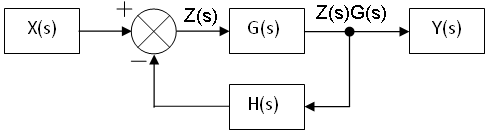
\includegraphics[width=\linewidth]{figs/Closed_Loop_Block_Deriv.png}
  \caption{Closed loop block diagram \cite{bib:closed_loop_block_derivation}}
  \label{fig:closed_loop_deriv}
\end{figure}

\begin{align}
  Y(s) &= Z(s) G(s) \nonumber \\
  Z(s) &= X(s) - Y(s) H(s) \nonumber \\
  X(s) &= Z(s) + Y(s) H(s) \nonumber \\
  X(s) &= Z(s) + Z(s) G(s) H(s) \nonumber \\
  \frac{Y(s)}{X(s)} &= \frac{Z(s) G(s)}{Z(s) + Z(s) G(s) H(s)} \nonumber \\
  \frac{Y(s)}{X(s)} &= \frac{G(s)}{1 + G(s) H(s)}
\end{align}

\noindent A more general form is

\begin{equation}
  \frac{Y(s)}{X(s)} = \frac{G(s)}{1 \mp G(s) H(s)}
\end{equation}

\noindent where positive feedback uses the top sign and negative feedback uses
the bottom sign.

\section{Kalman filter as Luenberger observer} \label{sec:app_kalman_luenberger}

\noindent A Luenberger observer is defined as

\begin{align}
  \mtx{x}_{k+1}^+ &= \mtx{A} \mtx{x}_k^- + \mtx{B} \mtx{u}_k + \mtx{L}
    (\mtx{y}_k - \hat{\mtx{y}}_k) \label{eq:luenberger1} \\
  \hat{\mtx{y}}_k &= \mtx{C} \mtx{x}_k^- \label{eq:luenberger2} \\ \nonumber
\end{align}

\noindent where a superscript of minus denotes a priori and plus denotes a
posteriori estimate. Combining equation (\ref{eq:luenberger1}) and equation
(\ref{eq:luenberger2}) gives
\\
\begin{equation} \label{eq:luenberger}
  \mtx{x}_{k+1}^+ = \mtx{A} \mtx{x}_k^- + \mtx{B} \mtx{u}_k + \mtx{L}
    (\mtx{y}_k - \mtx{C} \mtx{x}_k^-) \\
\end{equation}
\\
\noindent The following is a Kalman filter that considers the current update
step and the next predict step together rather than the current predict step and
current update step.

\begin{align}
  \text{Update step} \nonumber \\
  \mtx{K}_k &= \mtx{P}_k^- \mtx{H}^T (\mtx{H}\mtx{P}_k^- \mtx{H}^T +
    \mtx{R})^{-1} \\
  \mtx{x}_k^+ &= \mtx{x}_k^- + \mtx{K}_k (\mtx{y}_k - \mtx{H} \mtx{x}_k^-)
    \label{eq:post2_x} \\
  \mtx{P}_k^+ &= (\mtx{I} - \mtx{K}_k\mtx{H})\mtx{P}_k^- \\
  \text{Predict step} \nonumber \\
  \mtx{x}_{k+1}^+ &= \mtx{A} \mtx{x}_k^+ + \mtx{B} \mtx{u}_k
    \label{eq:pre2_x} \\
  \mtx{P}_{k+1}^- &= \mtx{A} \mtx{P}_k^+ \mtx{A}^T +
    \mtx{\Gamma}\mtx{Q}\mtx{\Gamma}^T
\end{align}
\\
\noindent Substitute equation (\ref{eq:post2_x}) into equation
(\ref{eq:pre2_x}).

\begin{align*}
  \mtx{x}_{k+1}^+ &= \mtx{A} (\mtx{x}_k^- +
    \mtx{K}_k (\mtx{y}_k - \mtx{H} \mtx{x}_k^-)) + \mtx{B} \mtx{u}_k \\
  \mtx{x}_{k+1}^+ &= \mtx{A} \mtx{x}_k^- +
    \mtx{A} \mtx{K}_k (\mtx{y}_k - \mtx{H} \mtx{x}_k^-) + \mtx{B} \mtx{u}_k \\
  \mtx{x}_{k+1}^+ &= \mtx{A} \mtx{x}_k^- + \mtx{B} \mtx{u}_k +
    \mtx{A} \mtx{K}_k (\mtx{y}_k - \mtx{H} \mtx{x}_k^-) \\
\end{align*}

\noindent Let $\mtx{C} = \mtx{H}$ and $\mtx{L} = \mtx{A} \mtx{K}_k$.

\begin{equation} \label{eq:app_kalman_leunberger}
  \mtx{x}_{k+1}^+ = \mtx{A} \mtx{x}_k^- + \mtx{B} \mtx{u}_k +
    \mtx{L} (\mtx{y}_k - \mtx{C} \mtx{x}_k^-) \\
\end{equation}
\\
\noindent which matches equation (\ref{eq:luenberger}). Therefore,
the eigenvalues of the Kalman filter observer can be obtained by

\begin{align}
  &eig(\mtx{A} - \mtx{L}\mtx{C}) \nonumber \\
  &eig(\mtx{A} - (\mtx{A}\mtx{K}_k)(\mtx{H})) \nonumber \\
  &eig(\mtx{A}(\mtx{I} - \mtx{K}_k\mtx{H}))
\end{align}

\bibliographystyle{IEEEtran}
\bibliography{state-space-guide.bib}
\glsaddall
\printglossaries
\end{document}
